\documentclass{ctexart}
\usepackage{graphicx}
\usepackage{caption}
\usepackage{float}
\usepackage{amsmath}
\usepackage{fancyhdr}
\usepackage{xunicode-addon}
\usepackage{booktabs}
\usepackage{listings}
\usepackage{hyperref}
\usepackage{longtable}
\usepackage[a4paper,hmargin=1.25in,vmargin=1in]{geometry}
% !TeX program = xelatex
\lstdefinestyle{mystyle}{
  basicstyle=\ttfamily\footnotesize,
  breakatwhitespace=false,         
  breaklines=true,                 
  captionpos=b,                    
  keepspaces=true,                 
  numbers=left,                    
  numbersep=5pt,                  
  showspaces=false,                
  showstringspaces=false,
  showtabs=false,                  
  tabsize=2
}

\lstset{style=mystyle}

\title{\begin{figure}[H]
	\centering 
	\includegraphics[height=7cm,width=14cm]{E:/Pictures/中科大.jpg}
	\end{figure}\Huge\textbf{图书馆管理系统课程设计报告}}
\date{}
\punctstyle{banjiao} 
\pagestyle{fancy}
	\fancyhead[C]{\LARGE\textbf{图书馆管理系统}}
	\fancyhead[L]{}
	\fancyhead[R]{}
	\fancyfoot[C]{\thepage}
\begin{document}
	\maketitle
	\thispagestyle{empty}
	
	\[\makebox{\Large{姓名:\underline{\makebox[5cm]{高茂航、李宇湘}}}}\]
	
	$$\makebox{\Large{日期:\underline{\makebox[5cm]{2024.7.20}}}}$$
	
	\clearpage

	\pagenumbering{arabic}

	\section{}
	
	
	
	\section{}

	
	
	\section{数据库概念结构设计}
	\begin{figure}[H]
		\centering 
		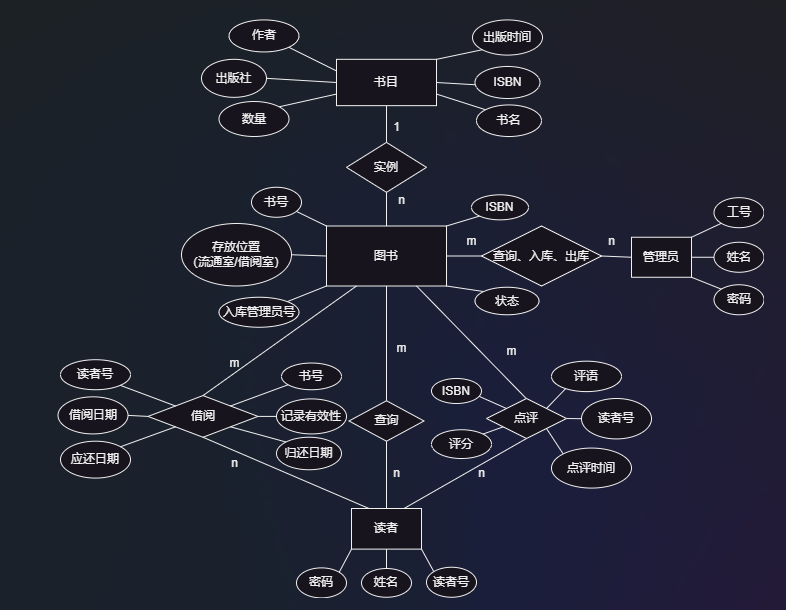
\includegraphics[height=10cm,width=12cm]{ER.png}
		\caption{ER图}
	\end{figure}

	\section{数据库逻辑结构设计(models.py)}
	\subsection{数据库表结构}
	\begin{longtable}{p{3.5cm}p{3.5cm}p{5.5cm}}
		\toprule
		\textbf{表名 (表名含义)} & \textbf{列名 (注释)} & \textbf{数据类型} \\
		\midrule
		\endhead
		dzTable (读者表) & \underline{dzid} (读者ID) & AutoField \\
		& psw (密码) & CharField(max\_length=256) \\
		& xm (姓名) & CharField(max\_length=10) \\
		\midrule
		tsglyTable (图书管理员表) & \underline{glyid} (管理员ID) & CharField(max\_length=10) \\
		& psw (密码) & CharField(max\_length=256) \\
		& xm (姓名) & CharField(max\_length=10) \\
		\midrule
		smTable (书目表) & \underline{isbn} & CharField(max\_length=50) \\
		& sm (书名) & CharField(max\_length=50) \\
		& zz (作者) & CharField(max\_length=50) \\
		& cbs (出版社) & CharField(max\_length=50) \\
		& cbny (出版时间) & DateTimeField \\
		& count (数量) & IntegerField(default=0) \\
		\midrule
		tsTable (图书实例表) & \underline{tsid} (图书ID) & AutoField \\
		& isbn (对应书目) & ForeignKey(smTable) \\
		& cfwz (存放位置) & CharField(max\_length=20) \\
		& zt (状态) & CharField(max\_length=20) \\
		& jbr (入库该书管理员工号) & ForeignKey(tsglyTable) \\
		\midrule
		BookReview (书评表) & \underline{dzid} (读者ID) & ForeignKey(dzTable) \\
		& \underline{isbn}& ForeignKey(smTable) \\
		& score (评分) & IntegerField(validators=[0,10]) \\
		& comment (评论) & TextField(max\_length=300, null=True) \\
		& comment\_time (评论时间) & DateTimeField(auto\_now\_add=True) \\
		\midrule
		jsTable (借书表) & \underline{dzid} (读者ID) & ForeignKey(dzTable) \\
		& \underline{tsid} (图书ID) & ForeignKey(tsTable, null=True) \\
		& \underline{jysj} (借阅时间) & DateTimeField \\
		& yhsj (应还时间) & DateTimeField \\
		& ghsj (归还时间) & DateTimeField(null=True) \\
		& is\_valid (记录是否有效) & BooleanField(default=True) \\
		\bottomrule
		\end{longtable}
		\subsection{具体分析}

		\subsubsection{dzTable (读者表)}
\begin{itemize}
    \item \textbf{结构}: 包含读者ID(主码)、密码、姓名。
    \item \textbf{解释}: 此表用于存储图书馆读者的基本信息。
    \item \textbf{3NF分析}: 满足3NF,因为每个非主属性完全函数依赖于主码(读者ID),不存在传递依赖或部分依赖。
    \item \textbf{BCNF分析}: 满足BCNF,由于不存在非主属性对主码的部分或传递依赖,同时每个候选码也是超码。
    \item \textbf{4NF分析}: 满足4NF,因为表中不存在多值依赖。
\end{itemize}

\subsubsection{tsglyTable (图书管理员表)}
\begin{itemize}
    \item \textbf{结构}: 包含管理员ID(主码)、密码、姓名。
    \item \textbf{解释}: 此表用于存储图书管理员的基本信息。
    \item \textbf{3NF分析}: 满足3NF,每个非主属性完全函数依赖于主码(管理员ID),不存在传递依赖或部分依赖。
    \item \textbf{BCNF分析}: 满足BCNF,因为不存在非主属性对主码的部分或传递依赖,且每个候选码也是超码。
    \item \textbf{4NF分析}: 满足4NF,因为表中不存在多值依赖。
\end{itemize}

\subsubsection{smTable (书目表)}
\begin{itemize}
    \item \textbf{结构}: 包含ISBN(主码)、书名、作者、出版社、出版时间、数量。
    \item \textbf{解释}: 此表记录了馆藏每个ISBN的书目的详细信息。
    \item \textbf{3NF分析}: 满足3NF,因为每个非主属性完全函数依赖于主码(ISBN),不存在传递依赖或部分依赖。
    \item \textbf{BCNF分析}: 满足BCNF,因为不存在非主属性对主码的部分或传递依赖,且每个候选码也是超码。
    \item \textbf{4NF分析}: 满足4NF,因为表中不存在多值依赖。
\end{itemize}

\subsubsection{tsTable (图书实例表)}
\begin{itemize}
    \item \textbf{结构}: 包含图书ID(主码)、该书的ISBN、存放位置(流通室/阅览室)、状态(不外借/未借出/已借出)、经办人。
    \item \textbf{解释}: 此表记录了图书馆中每本图书的具体信息。
    \item \textbf{3NF分析}: 满足3NF,因为每个非主属性完全函数依赖于主码(图书ID),不存在传递依赖或部分依赖。
    \item \textbf{BCNF分析}: 满足BCNF,因为不存在非主属性对主码的部分或传递依赖,且每个候选码也是超码。
    \item \textbf{4NF分析}: 满足4NF,因为表中不存在多值依赖。
\end{itemize}

\subsubsection{BookReview (书评表)}
\begin{itemize}
    \item \textbf{结构}: 包含读者ID、ISBN、评分、评论、评论时间,其中读者ID和ISBN共同构成复合主码。
    \item \textbf{解释}: 此表用于存储读者对图书的评分和评论。
    \item \textbf{3NF分析}: 满足3NF,因为每个非主属性完全函数依赖于复合主码(读者ID和ISBN),不存在传递依赖或部分依赖。
    \item \textbf{BCNF分析}: 满足BCNF,因为不存在非主属性对复合主码的部分或传递依赖,且每个候选码也是超码。
    \item \textbf{4NF分析}: 满足4NF,因为表中不存在多值依赖。
\end{itemize}

\subsubsection{jsTable (借书表)}
\begin{itemize}
    \item \textbf{结构}: 包含读者ID、图书ID、借阅时间、应还时间、归还时间、记录是否有效,其中读者ID、图书ID和借阅时间共同构成复合主码。
    \item \textbf{解释}: 此表记录了读者借阅图书的详细信息,其中记录是否有效表示借过的书是否仍在库,这样可以避免将借过的书出库后借书记录丢失。
    \item \textbf{3NF分析}: 满足3NF,因为每个非主属性完全函数依赖于复合主码(读者ID、图书ID和借阅时间),不存在传递依赖或部分依赖。
    \item \textbf{BCNF分析}: 满足BCNF,因为不存在非主属性对复合主码的部分或传递依赖,且每个候选码也是超码。
    \item \textbf{4NF分析}: 满足4NF,因为表中不存在多值依赖。
\end{itemize}

\subsection{总结}
所有表均满足第三范式(3NF)和BCNF的要求,
因为它们的每个非主属性都直接依赖于主码(或复合主码),
并且不存在任何传递依赖或部分依赖。此外,所有表也满足第四范式(4NF),
因为它们的表结构比较简单,不存在多值依赖。这样的设计确保了数据的一致性、减少了数据冗余,并且提高了查询效率。
	\section{数据库物理结构设计}
	数据库的物理设计一般依赖于相应的数据库管理系统,由系统自主完成,不用程序员过多考虑,但有时为了效率的问题或其他的要求,必须进行相应的物理设计(包括建立索引),以达到相应的要求。
	由于本图书馆管理系统的数据库表结构较为简单,且目前数据不多,因此暂未建立索引或进行其他物理结构设计,仅使用默认操作。


                            
	\section{后端功能设计与实现(views.py)}
	\subsection{home 函数}
	\subsection{home 函数}
	\begin{enumerate}
        \item \textbf{功能:} home 函数的主要功能是渲染并返回主页模板,处理对网站主页的请求;
        \item \textbf{实现逻辑}:
        \begin{enumerate}
            \item 接收一个请求对象作为参数;
            \item 使用 Django 的 \texttt{render} 函数,将请求对象和指定的模板('home.html')作为参数传递;
            \item 返回渲染后的 HTML 页面给用户。
        \end{enumerate}
    \end{enumerate}
    
    \subsection{login\_view 函数}
    \begin{enumerate}
        \item \textbf{功能:} login\_view 函数处理用户登录逻辑,支持两种用户类型:读者和管理员。根据用户类型和提供的凭证(用户名和密码),进行相应的身份验证,并根据验证结果重定向到不同的页面或返回错误信息;
        \item \textbf{实现逻辑}:
        \begin{enumerate}
            \item 初始化一个空字典 \texttt{context} 用于存储模板变量;
            \item 检查请求方法是否为 POST。如果不是,直接渲染并返回主页模板;
            \item 从 POST 请求中获取用户名、密码和用户类型;
            \item 验证用户名和密码是否提供。如果任一未提供,设置错误消息并重新渲染主页模板,显示错误消息;
            \item 根据用户类型(管理员或读者)执行不同的逻辑:
            \begin{enumerate}
                \item 管理员:使用用户名查询 \texttt{tsglyTable} 表,检查密码是否匹配。如果登录成功,设置会话变量并重定向到管理员首页;
                \item 读者:使用用户名查询 \texttt{dzTable} 表,检查密码是否匹配。如果登录成功,设置会话变量并重定向到读者首页;
            \end{enumerate}
            \item 如果用户名或密码不匹配,设置错误消息并重新渲染主页模板,显示错误消息。
        \end{enumerate}
    \end{enumerate}
    在这个过程中,\texttt{context} 字典被用来传递模板变量(如错误消息),而 Django 的 session 机制被用来在登录成功后存储用户信息,以便于跨请求保持用户状态。
    \subsection{register 函数}
\begin{enumerate}
    \item \textbf{功能:} 此函数用于新用户注册账户;
    \item \textbf{实现逻辑}:
    \begin{enumerate}
        \item 初始化一个空字典 \texttt{context} 用于存储传递给模板的数据;
        \item 如果请求方法为 GET,返回注册页面模板;
        \item 如果请求方法为 POST,执行注册逻辑:
        \begin{enumerate}
            \item 从 POST 数据中获取用户输入的姓名(xm)、密码(mm)和密码确认(mmqr);
            \item 验证姓名、密码和密码确认是否都已填写,如果有任何一个未填写,则在 \texttt{context} 中设置错误消息并重新渲染注册页面;
            \item 验证两次输入的密码是否一致,如果不一致,则设置错误消息并重新渲染注册页面;
            \item 验证密码长度是否至少为六位,如果不是,则设置错误消息并重新渲染注册页面;
            \item 检查用户名是否已被使用,如果是,则设置错误消息并重新渲染注册页面;
            \item 如果用户名未被使用,计算新用户的 ID,创建新用户记录,并保存到数据库;
            \item 注册成功后,重定向到登录页面。
        \end{enumerate}
        \item 如果请求方法既不是 GET 也不是 POST,则返回注册页面模板。
    \end{enumerate}
\end{enumerate}

\subsection{logout\_view 函数}
\begin{enumerate}
    \item \textbf{功能:} 此函数用于处理读者和管理员的退出登录操作;
    \item \textbf{实现逻辑}:
    \begin{enumerate}
        \item 检查 session 中是否存在 \texttt{login\_type},如果存在,则清空 session;
        \item 重定向到网站主页。
    \end{enumerate}
\end{enumerate}
\subsection{dz\_index 函数:读者首页}
\begin{enumerate}
    \item \textbf{功能}:显示读者的首页信息,包括当前借阅、历史借阅记录、用户排名等;
    \item \textbf{实现逻辑}:
    \begin{enumerate}
        \item 验证用户登录类型是否为读者,如果不是,则重定向到主页;
        \item 初始化上下文字典 \texttt{context},并从会话中获取用户姓名和ID,存入上下文;
        \item 查询当前用户的所有借阅记录,并筛选出当前借阅记录(未归还的);
        \item 计算总用户数;
        \item 基于借阅数量计算当前用户的排名;
        \item 遍历所有借阅记录,提取书籍信息和借阅状态,存入列表 \texttt{grzt};
        \item 使用 \texttt{Paginator} 对 \texttt{grzt} 进行分页处理;
        \item 从请求中获取页码,获取对应的页面对象 \texttt{page\_obj},并将其及其他信息添加到上下文;
        \item 渲染并返回 \texttt{dz\_index.html} 页面。
    \end{enumerate}
\end{enumerate}

\subsection{current\_borrows\_view 函数:当前借阅书籍}
\begin{enumerate}
    \item \textbf{功能}:显示读者当前借阅的书籍;
    \item \textbf{实现逻辑}:
    \begin{enumerate}
        \item 验证用户登录类型是否为读者,如果不是,则重定向到主页;
        \item 初始化上下文字典 \texttt{context},并从会话中获取用户姓名和ID,存入上下文;
        \item 查询当前用户的所有未归还借阅记录;
        \item 遍历当前借阅记录,提取书籍信息和借阅状态,存入列表 \texttt{grzt};
        \item 使用 \texttt{Paginator} 对 \texttt{grzt} 进行分页处理;
        \item 从请求中获取页码,获取对应的页面对象 \texttt{page\_obj},并将其及其他信息添加到上下文;
        \item 渲染并返回 \texttt{current\_borrows.html} 页面。
    \end{enumerate}
\end{enumerate}

\subsection{book\_details 函数:书籍详情}
\begin{enumerate}
    \item \textbf{功能}:显示一本书的详细信息,包括书籍信息和书评;
    \item \textbf{实现逻辑}:
    \begin{enumerate}
        \item 使用 \texttt{isbn} 参数从 \texttt{tsTable} 表中过滤出书籍信息,存储在 \texttt{books\_info} 变量中;
        \item 使用 \texttt{isbn} 参数从 \texttt{BookReview} 表中过滤出评分,并计算平均值,如果没有评分则默认为 0,结果存储在 \texttt{average\_score} 变量中;
        \item 使用 \texttt{isbn} 参数从 \texttt{BookReview} 表中过滤出所有评论,存储在 \texttt{reviews} 变量中;
        \item 创建一个字典 \texttt{context},包含用户会话中的姓名和 ID,书籍信息,平均评分,和评论列表;
        \item 使用 \texttt{render} 函数渲染 \texttt{book\_details.html} 模板,并传递 \texttt{context} 字典.
    \end{enumerate}
\end{enumerate}
\subsection{dz\_smztcx 函数:读者书目状态查询}
\begin{enumerate}
    \item \textbf{功能}:允许读者查询书目状态,包括书籍的详细信息和书评提交功能;
    \item \textbf{实现逻辑}:
    \begin{enumerate}
        \item 验证用户登录类型是否为读者,如果不是,则重定向到主页;
        \item 初始化上下文字典 \texttt{context},并从会话中获取用户姓名和ID,存入上下文;
        \item 如果是POST请求且包含书评信息,则处理书评提交:
        \begin{enumerate}
            \item 从POST请求中获取ISBN码、评分和评论内容;
            \item 尝试根据ISBN码在 \texttt{smTable} 表中找到对应的书籍实例;
            \item 如果找到,则在 \texttt{BookReview} 表中创建一条新的书评记录,并返回成功消息;
            \item 如果未找到对应的书籍实例,则返回错误消息;
        \end{enumerate}
        \item 如果是GET请求,则直接渲染并返回 \texttt{dz\_smztcx.html} 页面;
        \item 如果是POST请求但不是提交书评的请求,则处理书目查询:
        \begin{enumerate}
            \item 从POST请求中获取书名、作者、ISBN码和出版社信息,并存入上下文;
            \item 如果书名为空,则返回错误消息并提示输入书名进行搜索;
            \item 使用提供的信息对 \texttt{smTable} 表进行过滤查询,实现模糊搜索;
            \item 遍历查询结果,提取每本书的详细信息和状态,存入列表 \texttt{smzt};
            \item 将 \texttt{smzt} 列表和其他信息添加到上下文;
            \item 渲染并返回 \texttt{dz\_smztcx.html} 页面。
        \end{enumerate}
    \end{enumerate}
\end{enumerate}

\subsection{check\_review 函数:检查是否已经评论过}
\begin{enumerate}
    \item \textbf{功能}:检查用户是否已经对某本书进行了评论;
    \item \textbf{实现逻辑}:
    \begin{enumerate}
        \item 从会话中获取用户ID;
        \item 使用用户ID和ISBN码查询 \texttt{BookReview} 表,检查是否存在评论记录;
        \item 如果存在评论记录,返回提示信息,说明用户已经评论过该书;
        \item 如果不存在评论记录,返回空消息,允许用户进行评论;
        \item 返回包含检查结果和消息的JSON响应。
    \end{enumerate}
\end{enumerate}

\subsection{submit\_review 函数:提交评论}
\begin{enumerate}
    \item \textbf{功能}:允许用户提交对书籍的评论;
    \item \textbf{实现逻辑}:
    \begin{enumerate}
        \item 检查请求方法是否为POST,如果不是,返回错误消息;
        \item 从POST请求中获取ISBN码、评分和评论内容;
        \item 从会话中获取用户ID;
        \item 如果评分为空,返回错误消息,说明评分是必填项;
        \item 尝试根据ISBN码在 \texttt{smTable} 表中找到对应的书籍实例;
        \item 如果找到书籍实例,创建一条新的书评记录,并返回成功消息;
        \item 如果未找到书籍实例,返回错误消息,说明提供的ISBN码无效;
    \end{enumerate}
\end{enumerate}

\subsection{dz\_js 函数:读者借书}
\begin{enumerate}
    \item \textbf{功能}:实现读者借书的功能;
    \item \textbf{实现逻辑}:
    \begin{enumerate}
        \item 验证用户登录类型是否为读者,如果不是,则重定向到主页;
        \item 初始化上下文字典 \texttt{context},并从会话中获取用户姓名和ID,存入上下文;
        \item 如果是GET请求,直接渲染并返回 \texttt{dz\_js.html} 页面;
        \item 如果是POST请求,处理借书逻辑:
        \begin{enumerate}
            \item 从POST请求中获取ISBN码,并存入上下文;
            \item 如果ISBN码为空,返回错误消息并提示填写完整的ISBN号;
            \item 尝试根据ISBN码在 \texttt{smTable} 表中找到对应的书籍实例;
            \item 如果未找到书籍实例,返回错误消息,说明ISBN号填写错误;
            \item 检查当前用户的未归还借阅记录数是否已达上限;
            \item 如果已达上限,返回错误消息,说明借阅书籍数已达上限;
            \item 检查所选图书的状态是否为“未借出”;
            \item 如果所有图书已被借出,返回错误消息,说明无法借阅;
            \item 更新图书状态为“已借出”,并创建借书记录;
            \item 返回成功消息,提示借阅成功,并显示图书ID。
        \end{enumerate}
    \end{enumerate}
\end{enumerate}
\subsection{dz\_hs 函数:读者还书}
\begin{enumerate}
    \item \textbf{功能}:实现读者还书的功能;
    \item \textbf{实现逻辑}:
    \begin{enumerate}
        \item 验证用户登录类型是否为读者,如果不是,则重定向到主页;
        \item 初始化上下文字典 \texttt{context},并从会话中获取用户姓名和ID,存入上下文;
        \item 如果是GET请求,直接渲染并返回 \texttt{dz\_hs.html} 页面;
        \item 如果是POST请求,处理还书逻辑:
        \begin{enumerate}
            \item 从POST请求中获取图书ID,并存入上下文;
            \item 如果图书ID为空或不是数字,返回错误消息;
            \item 查询图书ID是否存在,如果不存在,返回错误消息;
            \item 查询该读者是否有未归还的借书记录,如果没有,返回错误消息;
            \item 检查图书是否逾期未还,如果逾期,计算并提示逾期费用;
            \item 更新图书状态为“未借出”,并记录归还时间;
            \item 返回成功消息,提示图书已归还。
        \end{enumerate}
    \end{enumerate}
\end{enumerate}

\subsection{my\_reviews 函数:读者评书记录}
\begin{enumerate}
    \item \textbf{功能}:显示读者的评书记录;
    \item \textbf{实现逻辑}:
    \begin{enumerate}
        \item 从会话中获取读者ID,并初始化上下文字典 \texttt{context};
        \item 查询当前读者的所有评书记录,并按评论时间排序;
        \item 使用 \texttt{Paginator} 对评书记录进行分页处理;
        \item 从请求中获取页码,获取对应的页面对象 \texttt{page\_obj},并将其及其他信息添加到上下文;
        \item 遍历分页后的评书记录,提取书籍信息、评分、评论内容等,存入列表;
        \item 渲染并返回 \texttt{my\_reviews.html} 页面。
    \end{enumerate}
\end{enumerate}

\subsection{revoke\_review 函数:撤销评论}
\begin{enumerate}
    \item \textbf{功能}:允许读者撤销自己的评论;
    \item \textbf{实现逻辑}:
    \begin{enumerate}
        \item 从POST请求的body中解析JSON数据,获取评论ID;
        \item 尝试根据评论ID找到对应的评论记录;
        \item 如果找到,删除该评论记录,并返回成功消息;
        \item 如果未找到或发生其他错误,返回错误消息。
    \end{enumerate}
\end{enumerate}
\subsection{ranking 函数:展示排名信息}
\begin{enumerate}
    \item \textbf{功能}:展示评分最高的十本书及其评分,以及被借阅次数最多的十本书及其被借次数。
    \item \textbf{实现逻辑}:
    \begin{enumerate}
        \item 验证用户登录类型是否为读者,如果不是,则重定向到主页;
        \item 初始化上下文字典 \texttt{context},并从会话中获取用户姓名和ID,存入上下文;
        \item 获取评分最高的十本书及其评分,确保书籍有评分,存入上下文;
        \item 获取被借阅次数最多的十本书及其被借次数,确保书籍被借阅过,存入上下文;
        \item 渲染并返回 \texttt{ranking.html} 页面,展示排名信息。
    \end{enumerate}
\end{enumerate}

\subsection{gly\_index 函数:管理员首页}
\begin{enumerate}
    \item \textbf{功能}:显示管理员首页。
    \item \textbf{实现逻辑}:
    \begin{enumerate}
        \item 验证用户登录类型是否为管理员,如果不是,则重定向到主页;
        \item 初始化上下文字典 \texttt{context},并从会话中获取管理员姓名和ID,存入上下文;
        \item 渲染并返回 \texttt{gly\_index.html} 页面,显示管理员首页。
    \end{enumerate}
\end{enumerate}

\subsection{book\_details2 函数:管理员页面书籍详情}
\begin{enumerate}
    \item \textbf{功能}:在管理员页面显示书籍的详细信息。
    \item \textbf{实现逻辑}:
    \begin{enumerate}
        \item 根据传入的ISBN查询书籍信息;
        \item 查询并计算书籍的平均评分;
        \item 查询书籍的所有评论;
        \item 初始化上下文字典 \texttt{context},并将查询到的信息存入上下文;
        \item 渲染并返回 \texttt{book\_details2.html} 页面,展示书籍详情。
    \end{enumerate}
\end{enumerate}

\subsection{gly\_smztcx 函数:管理员书目状态查询}
\begin{enumerate}
    \item \textbf{功能}:允许管理员根据书名、作者、ISBN、出版社等信息查询书目状态。
    \item \textbf{实现逻辑}:
    \begin{enumerate}
        \item 验证用户登录类型是否为管理员,如果不是,则重定向到主页;
        \item 初始化上下文字典 \texttt{context},并从会话中获取管理员姓名和ID,存入上下文;
        \item 如果是GET请求,直接渲染并返回 \texttt{gly\_smztcx.html} 页面;
        \item 如果是POST请求,处理书目状态查询逻辑:
        \begin{enumerate}
            \item 从POST请求中获取书名、作者、ISBN、出版社等信息;
            \item 如果书名为空,返回错误消息;
            \item 使用模糊搜索查询满足条件的书目,并计算每本书的在库册数、不外借册数、未借出册数、已借出册数;
            \item 将查询结果和其他信息存入上下文;
            \item 渲染并返回 \texttt{gly\_smztcx.html} 页面,展示查询结果。
        \end{enumerate}
    \end{enumerate}
\end{enumerate}
\subsection{smzt\_all 函数:所有书目状态查询}
\begin{enumerate}
    \item \textbf{功能}:显示所有书目的状态信息;
    \item \textbf{实现逻辑}:
    \begin{enumerate}
        \item 初始化上下文字典 \texttt{context},并从会话中获取管理员ID,存入上下文;
        \item 查询所有书目的信息;
        \item 遍历查询结果,对每本书进行以下操作:
        \begin{enumerate}
            \item 提取书目的基本信息(ISBN、书名、作者、出版社、出版年月);
            \item 查询并计算该书目的库存总数、不外借数量、未借出数量、已借出数量;
            \item 将上述信息存入列表 \texttt{smzt} 中;
        \end{enumerate}
        \item 使用 \texttt{Paginator} 对 \texttt{smzt} 进行分页处理,每页显示10个书目;
        \item 从请求中获取页码,获取对应的页面对象 \texttt{page\_obj},并将其及其他信息添加到上下文;
        \item 渲染并返回 \texttt{smzt\_all.html} 页面。
    \end{enumerate}
\end{enumerate}

\subsection{borrowed\_books 函数:所有借阅信息}
\begin{enumerate}
    \item \textbf{功能}:显示所有当前借阅信息;
    \item \textbf{实现逻辑}:
    \begin{enumerate}
        \item 验证用户登录类型是否为管理员,如果不是,则重定向到主页;
        \item 初始化上下文字典 \texttt{context},并从会话中获取用户姓名和ID,存入上下文;
        \item 查询所有当前未归还的借阅记录,并按读者ID排序;
        \item 将查询结果存入上下文;
        \item 渲染并返回 \texttt{borrowed\_books.html} 页面。
    \end{enumerate}
\end{enumerate}

\subsection{gly\_rk 函数:管理员入库}
\begin{enumerate}
    \item \textbf{功能}:管理员进行书籍入库操作;
    \item \textbf{实现逻辑}:
    \begin{enumerate}
        \item 验证用户登录类型是否为管理员,如果不是,则重定向到主页;
        \item 初始化上下文字典 \texttt{context},并从会话中获取用户姓名和ID,存入上下文;
        \item 如果请求方法为GET,直接渲染并返回 \texttt{gly\_rk.html} 页面;
        \item 如果请求方法为POST,执行以下操作:
        \begin{enumerate}
            \item 从请求中获取ISBN、入库数量、入库后状态、书名、作者、出版社、出版年月等信息,并存入上下文;
            \item 验证必要信息的完整性,不完整则返回错误信息;
            \item 根据ISBN查询书目,判断是旧书入库还是新书入库;
            \item 对于旧书入库,进一步验证书名、作者、出版社、出版年月的匹配性,不匹配则返回错误信息;
            \item 根据入库后状态(流通室、阅览室),创建相应数量的图书实例,并保存;
            \item 更新书目的库存总数,并保存;
            \item 设置成功信息,并可能刷新页面;
            \item 渲染并返回 \texttt{gly\_rk.html} 页面,显示操作结果。
        \end{enumerate}
    \end{enumerate}
\end{enumerate}
\subsection{gly\_ck 函数:管理员出库}
\begin{enumerate}
    \item \textbf{功能}:管理员进行书籍出库操作;
    \item \textbf{实现逻辑}:
    \begin{enumerate}
        \item 验证用户登录类型是否为管理员,如果不是,则重定向到主页;
        \item 初始化上下文字典 \texttt{context},并从会话中获取用户姓名和ID,存入上下文;
        \item 如果请求方法为GET,直接渲染并返回 \texttt{gly\_ck.html} 页面;
        \item 如果请求方法为POST,执行以下操作:
        \begin{enumerate}
            \item 从请求中获取ISBN、出库数量、出库优先位置,并存入上下文;
            \item 验证必要信息的完整性,不完整则返回错误信息;
            \item 验证出库优先位置是否合法(流通室或阅览室),不合法则返回错误信息;
            \item 根据ISBN查询书目,如果不存在则返回错误信息;
            \item 计算未借出和不外借的图书数量,以及所有图书数量;
            \item 如果出库数量超过藏书总数或可出库数量,返回错误信息;
            \item 根据出库优先位置,优先出库未借出或不外借的图书;
            \item 更新图书状态为无效,并删除图书记录;
            \item 更新书目的库存总数,如果没有剩余的书,则删除书目记录;
            \item 设置成功信息,并返回出库成功的图书ID;
            \item 渲染并返回 \texttt{gly\_ck.html} 页面,显示操作结果。
        \end{enumerate}
    \end{enumerate}
\end{enumerate}

\subsection{book\_count\_view 函数:书籍借阅次数统计}
\begin{enumerate}
    \item \textbf{功能}:统计并显示各书籍的借阅次数;
    \item \textbf{实现逻辑}:
    \begin{enumerate}
        \item 从 \texttt{jsTable} 中查询每本书的ISBN、书名和借阅次数;
        \item 对查询结果按借阅次数降序排序;
        \item 将查询结果存入上下文字典 \texttt{context};
        \item 渲染并返回 \texttt{book\_count.html} 页面。
    \end{enumerate}
\end{enumerate}

\subsection{reader\_count\_view 函数:读者借阅次数统计}
\begin{enumerate}
    \item \textbf{功能}:统计并显示各读者的借阅次数;
    \item \textbf{实现逻辑}:
    \begin{enumerate}
        \item 从 \texttt{jsTable} 中查询每位读者的ID、姓名和借阅次数;
        \item 对查询结果按借阅次数降序排序;
        \item 将查询结果存入上下文字典 \texttt{context};
        \item 渲染并返回 \texttt{reader\_count.html} 页面。
    \end{enumerate}
\end{enumerate}
	\section{}
	\section{}
	\section{}
	\section{}
	\section{}
	\section{}

	

\end{document}